\documentclass[preprint,12pt,aps,pra,showkeys,amsmath,amssymb,superscriptaddress,floatfix]{revtex4-2}
\usepackage[T1]{fontenc}
\usepackage[utf8]{inputenc}
\usepackage{amsmath,amssymb,amsthm,mathtools,mathrsfs}
\usepackage{microtype,booktabs,enumitem}
\usepackage{xcolor,tikz,etoolbox}
\usepackage[skins,breakable]{tcolorbox}
\usepackage{needspace}
% Keep diagram geometry independent of REVTeX preprint body spacing.
\AtBeginEnvironment{tikzpicture}{\linespread{1}\selectfont}
\usetikzlibrary{arrows.meta,positioning,calc,fit,decorations.pathreplacing}
\usepackage{graphicx}
\usepackage{hyperref}

\definecolor{MMBlue}{RGB}{0,82,155}
\definecolor{MMOrange}{RGB}{200,80,0}
\tikzset{
 mmnode/.style={draw=MMBlue,rounded corners=2pt,fill=MMBlue!4,align=left,execute at begin node={\raggedright},text width=5cm,font=\fontsize{10}{12}\selectfont,inner sep=6pt},
 mmimport/.style={mmnode,draw=black!65,fill=black!4},
 mmcandidate/.style={mmnode,draw=MMOrange,dashed,fill=MMOrange!5},
 mmrejected/.style={mmnode,draw=black,densely dotted,fill=black!8},
 mmproof/.style={->,thick,MMBlue},
 mmflow/.style={->,semithick,black!70},
 mmrepair/.style={->,dashed,thick,MMOrange},
 mmcandidatearrow/.style={->,dashed,semithick,MMOrange},
 mmnote/.style={font=\scriptsize,fill=white,inner sep=2pt,align=center}}

\usepackage[section]{placeins}
\setlength{\emergencystretch}{3em}
\setlist{itemsep=3pt,topsep=4pt}
\newtheorem{theorem}{Theorem}[section]
\newtheorem{proposition}[theorem]{Proposition}
\newtheorem{lemma}[theorem]{Lemma}
\newtheorem{corollary}[theorem]{Corollary}
\theoremstyle{definition}
\newtheorem{definition}[theorem]{Definition}
\newtheorem{example}[theorem]{Example}
\theoremstyle{remark}
\newtheorem{remark}[theorem]{Remark}
% Avoid isolated statement headings and single-line paragraph fragments.
\BeforeBeginEnvironment{theorem}{\Needspace{6\baselineskip}}
\BeforeBeginEnvironment{definition}{\Needspace{5\baselineskip}}
\BeforeBeginEnvironment{proposition}{\Needspace{5\baselineskip}}
\BeforeBeginEnvironment{lemma}{\Needspace{5\baselineskip}}
\BeforeBeginEnvironment{corollary}{\Needspace{5\baselineskip}}
\clubpenalty=5000
\widowpenalty=5000
\newcommand{\R}{\mathbb R}\newcommand{\Z}{\mathbb Z}\newcommand{\N}{\mathbb N}
\newcommand{\Pa}{\operatorname{Pa}}\newcommand{\Desc}{\operatorname{Desc}}
\newcommand{\cl}{\operatorname{cl}}\newcommand{\cost}{\operatorname{cost}}
\newcommand{\status}{\operatorname{status}}
% Faculty cards: a visual rail groups the five faculties within one agent.
% The rail has no arrowhead and does not represent a proof dependency.
\newcommand{\mmfacultybadge}[1]{%
 \node[circle,draw=MMBlue,line width=1pt,fill=white,
 minimum size=7mm,inner sep=0pt,font=\sffamily\small\bfseries,text=MMBlue]
 at ([xshift=15pt,yshift=-15pt]frame.north west) {#1};}
\newcommand{\mmfacultyrail}{%
 \draw[MMBlue!80,line width=1pt]
 ([xshift=15pt,yshift=2pt]frame.north west)--
 ([xshift=15pt,yshift=-2pt]frame.south west);}
\newtcolorbox{mmfacultybox}[2]{enhanced,breakable,
 colback=MMBlue!4,colframe=MMBlue!4,boxrule=0pt,arc=3pt,
 left=39pt,right=9pt,top=4pt,bottom=4pt,
 before skip=2pt,after skip=2pt,
 fontupper=\small\linespread{1.1}\selectfont,
 overlay unbroken={\mmfacultyrail\mmfacultybadge{#1}},
 overlay first={\mmfacultyrail\mmfacultybadge{#1}},
 overlay middle={\mmfacultyrail},overlay last={\mmfacultyrail}}
\newcommand{\mmfaculty}[3]{%
 \begin{mmfacultybox}{#1}{#2}
 {\sffamily\bfseries\color{MMBlue}#2}\par\smallskip #3
 \end{mmfacultybox}}
\newcommand{\agent}[9]{%
 \Needspace{8\baselineskip}
 \subsubsection{#1}
 \noindent\textbf{Object.} #2\par
 \noindent\textbf{Role.} #3\par\smallskip
 \mmfaculty{E}{Ego}{#4}
 \mmfaculty{M}{Memory}{#5}
 \mmfaculty{I}{Intellect}{#6}
 \mmfaculty{S}{Sense}{#7}
 \mmfaculty{A}{Action}{#8}
 \smallskip\noindent #9\par}

\usepackage{longtable,array,calc}
\providecommand{\tightlist}{\setlength{\itemsep}{2pt}\setlength{\parskip}{0pt}}
\makeatletter
\def\frontmatter@abstract@produce{\par\addvspace{\frontmatter@preabstractspace}%
\begingroup\prep@absbox\unvbox\absbox\post@absbox\endgroup
\addvspace{\frontmatter@postabstractspace}}
\makeatother
\newcommand{\field}[2]{\par\smallskip\noindent\textbf{#1.} #2\par}
\setlength{\emergencystretch}{5em}
\AtBeginEnvironment{verbatim}{\small\linespread{1.0}\selectfont}


\hypersetup{colorlinks=true,linkcolor=MMBlue,urlcolor=MMBlue,pdfauthor={Dibakar Sigdel}}

\begin{document}

\title{Compact-to-Hausdorff Continuous Bijection Theorem\\[4pt]\large An End-to-End Meta-Math Walkthrough}

\author{Dibakar Sigdel}

\affiliation{Mindverse Computing LLC, Lynnwood, WA 98087, USA}

\date{October 2026}

\begin{abstract}

A complete authored walkthrough of compact-to-hausdorff continuous
bijection theorem, with explicit mathematical contracts, local
verification gates, and reusable exports. The report presents the target
theorem, declared imports, a dependency graph, five-faculty node
contracts, a continuous proof, a worked example, and a hypothesis-repair
audit. It is an authored mathematical exposition, not a deployed-agent
transcript or a formal proof-assistant certificate.

\end{abstract}\maketitle\linespread{1.12}\selectfont

\noindent\textbf{GT-02 / General Topology / Report v1}

\section{Target and import contract}

\begin{theorem}

If X is compact, Y is Hausdorff, and \(f:X\to Y\) is a continuous
bijection, then f is a homeomorphism.

A homeomorphism is a bijection continuous in both directions. The task
is therefore to prove continuity of the inverse. The source X need not
initially be assumed Hausdorff; the conclusion makes it homeomorphic to
a Hausdorff space.

\end{theorem}

\subsection{Foundations and permitted imports}

compactness means every open cover has a finite subcover. Hausdorff
means distinct points have disjoint open neighborhoods. A closed map
sends closed subsets to closed subsets. The proof below derives the
supporting compactness lemmas directly from these definitions.

For the final application only, import compactness of the closed
interval, the quotient universal property, and
\(e^{2\pi it}=e^{2\pi is}\) exactly when \(t-s\in\mathbb Z\).

\clearpage\section{Node interaction workflow}

\begin{center}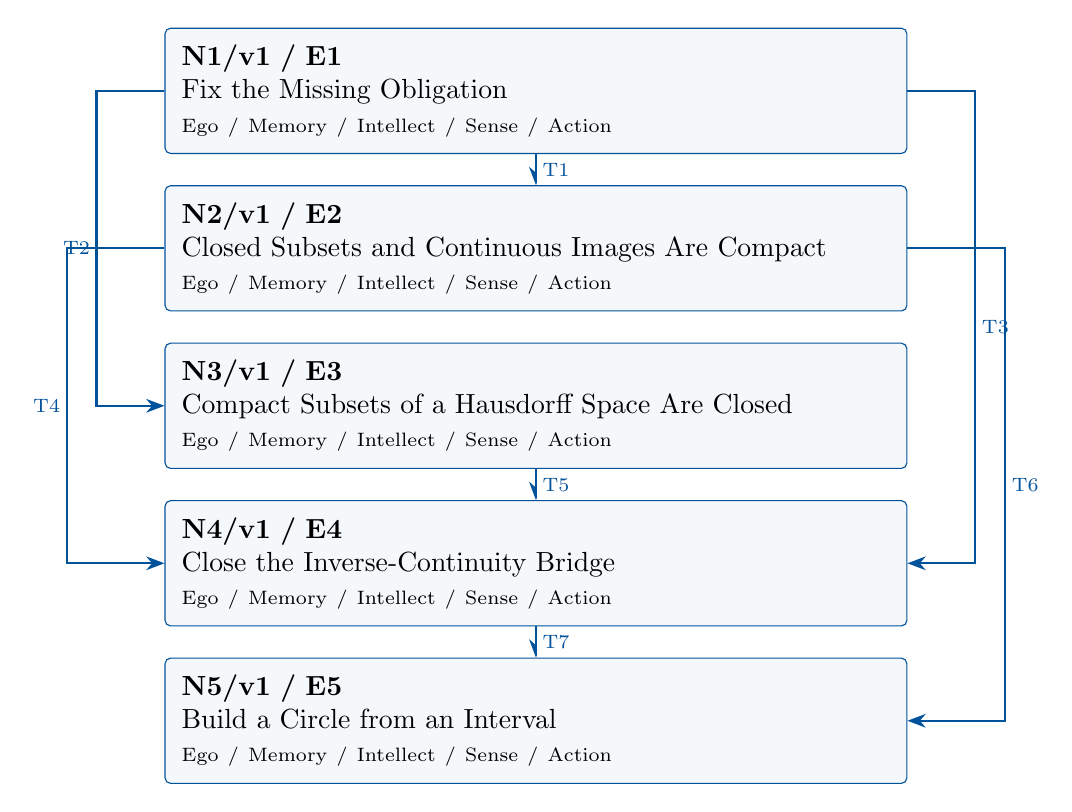
\begin{tikzpicture}[>=Stealth,x=1cm,y=1cm]

\node[mmnode,text width=9cm,minimum height=1.25cm] (N1) at (0,0.0) {\textbf{N1/v1 / E1}\\Fix the Missing Obligation\\{\scriptsize Ego / Memory / Intellect / Sense / Action}};

\node[mmnode,text width=9cm,minimum height=1.25cm] (N2) at (0,-2.0) {\textbf{N2/v1 / E2}\\Closed Subsets and Continuous Images Are Compact\\{\scriptsize Ego / Memory / Intellect / Sense / Action}};

\node[mmnode,text width=9cm,minimum height=1.25cm] (N3) at (0,-4.0) {\textbf{N3/v1 / E3}\\Compact Subsets of a Hausdorff Space Are Closed\\{\scriptsize Ego / Memory / Intellect / Sense / Action}};

\node[mmnode,text width=9cm,minimum height=1.25cm] (N4) at (0,-6.0) {\textbf{N4/v1 / E4}\\Close the Inverse-Continuity Bridge\\{\scriptsize Ego / Memory / Intellect / Sense / Action}};

\node[mmnode,text width=9cm,minimum height=1.25cm] (N5) at (0,-8.0) {\textbf{N5/v1 / E5}\\Build a Circle from an Interval\\{\scriptsize Ego / Memory / Intellect / Sense / Action}};

\draw[mmproof] (N1.south) -- node[mmnote,right] {T1} (N2.north);

\draw[mmproof] (N1.west) -- (-5.58,0) -- node[mmnote,left] {T2} (-5.58,-4) -- (N3.west);

\draw[mmproof] (N1.east) -- (5.58,0) -- node[mmnote,right] {T3} (5.58,-6) -- (N4.east);

\draw[mmproof] (N2.west) -- (-5.96,-2) -- node[mmnote,left] {T4} (-5.96,-6) -- (N4.west);

\draw[mmproof] (N3.south) -- node[mmnote,right] {T5} (N4.north);

\draw[mmproof] (N2.east) -- (5.96,-2) -- node[mmnote,right] {T6} (5.96,-8) -- (N5.east);

\draw[mmproof] (N4.south) -- node[mmnote,right] {T7} (N5.north);

\end{tikzpicture}\end{center}

Each box is one mathematical agent containing all five faculties. Blue
arrows carry the versioned exports listed below. The layout gives a
reading order; only drawn arrows assert dependencies. Diagnostic repair
is separate from the proof DAG.

\clearpage\subsection{Versioned evidence-transfer ledger}

\begingroup\small\linespread{1.05}\selectfont

\Needspace{5\baselineskip}\field{T1: N1/E1/v1 to N2}{The inverse set-map \(h=f^{-1}:Y\to X\) exists; it remains to prove its
continuity.}

\field{Receiving activity}{N2: Closed Subsets and Continuous Images Are Compact}

\field{Compatibility}{Use the same mathematical objects and hypotheses as the source export.
Receiving contract: N1/E1 and the open-cover definition of compactness.}

\Needspace{5\baselineskip}\field{T2: N1/E1/v1 to N3}{The inverse set-map \(h=f^{-1}:Y\to X\) exists; it remains to prove its
continuity.}

\field{Receiving activity}{N3: Compact Subsets of a Hausdorff Space Are Closed}

\field{Compatibility}{Use the same mathematical objects and hypotheses as the source export.
Receiving contract: N1/E1 supplies the Hausdorff target; take an
arbitrary compact subset \(K\subset Y\).}

\Needspace{5\baselineskip}\field{T3: N1/E1/v1 to N4}{The inverse set-map \(h=f^{-1}:Y\to X\) exists; it remains to prove its
continuity.}

\field{Receiving activity}{N4: Close the Inverse-Continuity Bridge}

\field{Compatibility}{Use the same mathematical objects and hypotheses as the source export.
Receiving contract: N1/E1, N2/E2, and N3/E3.}

\Needspace{5\baselineskip}\field{T4: N2/E2/v1 to N4}{For every closed \(C\subset X\), the image \(f(C)\) is compact.}

\field{Receiving activity}{N4: Close the Inverse-Continuity Bridge}

\field{Compatibility}{Use the same mathematical objects and hypotheses as the source export.
Receiving contract: N1/E1, N2/E2, and N3/E3.}

\Needspace{5\baselineskip}\field{T5: N3/E3/v1 to N4}{Every compact subset of a Hausdorff space is closed.}

\field{Receiving activity}{N4: Close the Inverse-Continuity Bridge}

\field{Compatibility}{Use the same mathematical objects and hypotheses as the source export.
Receiving contract: N1/E1, N2/E2, and N3/E3.}

\Needspace{5\baselineskip}\field{T6: N2/E2/v1 to N5}{For every closed \(C\subset X\), the image \(f(C)\) is compact.}

\field{Receiving activity}{N5: Build a Circle from an Interval}

\field{Compatibility}{Use the same mathematical objects and hypotheses as the source export.
Receiving contract: N2/E2, N4/E4, compactness of \([0,1]\), the quotient
topology, and the exponential circle parametrization.}

\Needspace{5\baselineskip}\field{T7: N4/E4/v1 to N5}{\(f\) is a homeomorphism.}

\field{Receiving activity}{N5: Build a Circle from an Interval}

\field{Compatibility}{Use the same mathematical objects and hypotheses as the source export.
Receiving contract: N2/E2, N4/E4, compactness of \([0,1]\), the quotient
topology, and the exponential circle parametrization.}

\endgroup

\clearpage\section{Agent roles and five-faculty activities}\begingroup\small\linespread{1.05}\selectfont\setlist{itemsep=1pt,topsep=2pt}

\subsection{N1/v1: Fix the Missing Obligation}

\field{Object and role}{Fix the Missing Obligation. Establish the following local result: The
inverse set-map \(h=f^{-1}:Y\to X\) exists; it remains to prove its
continuity.}

\field{Inputs}{\(X\) compact, \(Y\) Hausdorff, and \(f:X\to Y\) a continuous bijection.}

\mmfaculty{E}{Ego}{Own E1/v1: The inverse set-map \(h=f^{-1}:Y\to X\) exists; it remains to
prove its continuity.}

\mmfaculty{M}{Memory}{Bijection and topology definitions}

\mmfaculty{I}{Intellect}{Target inverse continuity}

\mmfaculty{S}{Sense}{Check each hypothesis separately}

\mmfaculty{A}{Action}{Carry out the numbered deductions and publish E1/v1 together with its
hypotheses and proof location.}

\smallskip\noindent\textbf{Numbered mathematical activities}

\begin{enumerate}[label=N1.\arabic*,leftmargin=3.4em]

\item Check compactness, Hausdorffness, continuity, and bijectivity
separately.

\item Define the inverse as a set-map.

\item Reduce inverse continuity to closed inverse images.

\end{enumerate}

\field{Export E1/v1}{The inverse set-map \(h=f^{-1}:Y\to X\) exists; it remains to prove its
continuity.}

\field{Acceptance gate}{Check each hypothesis separately Publish only after checking every
displayed deduction.}

\field{Targeted repair}{If the check fails, revise N1: Check each hypothesis separately Recheck
dependent nodes N2, N3, N4, N5.}

\clearpage

\subsection{N2/v1: Closed Subsets and Continuous Images Are Compact}

\field{Object and role}{Closed Subsets and Continuous Images Are Compact. Establish the
following local result: For every closed \(C\subset X\), the image
\(f(C)\) is compact.}

\field{Inputs}{N1/E1 and the open-cover definition of compactness.}

\mmfaculty{E}{Ego}{Own E2/v1: For every closed \(C\subset X\), the image \(f(C)\) is
compact.}

\mmfaculty{M}{Memory}{Open covers and preimages}

\mmfaculty{I}{Intellect}{Transfer finite-subcover property}

\mmfaculty{S}{Sense}{Use closed source sets}

\mmfaculty{A}{Action}{Carry out the numbered deductions and publish E2/v1 together with its
hypotheses and proof location.}

\smallskip\noindent\textbf{Numbered mathematical activities}

\begin{enumerate}[label=N2.\arabic*,leftmargin=3.4em]

\item Add the open complement of \(C\) to a cover and use compactness of
\(X\).

\item Pull an open cover of \(f(C)\) back along the restricted continuous map.

\item Push the resulting finite subcover forward.

\end{enumerate}

\field{Export E2/v1}{For every closed \(C\subset X\), the image \(f(C)\) is compact.}

\field{Acceptance gate}{Use closed source sets Publish only after checking every displayed
deduction.}

\field{Targeted repair}{If the check fails, revise N2: Use closed source sets Recheck dependent
nodes N4, N5.}

\clearpage

\subsection{N3/v1: Compact Subsets of a Hausdorff Space Are Closed}

\field{Object and role}{Compact Subsets of a Hausdorff Space Are Closed. Establish the following
local result: Every compact subset of a Hausdorff space is closed.}

\field{Inputs}{N1/E1 supplies the Hausdorff target; take an arbitrary compact subset
\(K\subset Y\).}

\mmfaculty{E}{Ego}{Own E3/v1: Every compact subset of a Hausdorff space is closed.}

\mmfaculty{M}{Memory}{Disjoint neighborhoods}

\mmfaculty{I}{Intellect}{Separate outsider from compact set}

\mmfaculty{S}{Sense}{Use finite intersections after a finite subcover}

\mmfaculty{A}{Action}{Carry out the numbered deductions and publish E3/v1 together with its
hypotheses and proof location.}

\smallskip\noindent\textbf{Numbered mathematical activities}

\begin{enumerate}[label=N3.\arabic*,leftmargin=3.4em]

\item Separate an outsider from each point of \(K\) by disjoint open
neighborhoods.

\item Use compactness to select finitely many neighborhoods covering \(K\).

\item Intersect the finitely many outsider neighborhoods to prove the
complement open.

\end{enumerate}

\field{Export E3/v1}{Every compact subset of a Hausdorff space is closed.}

\field{Acceptance gate}{Use finite intersections after a finite subcover Publish only after
checking every displayed deduction.}

\field{Targeted repair}{If the check fails, revise N3: Use finite intersections after a finite
subcover Recheck dependent nodes N4, N5.}

\clearpage

\subsection{N4/v1: Close the Inverse-Continuity Bridge}

\field{Object and role}{Close the Inverse-Continuity Bridge. Establish the following local
result: \(f\) is a homeomorphism.}

\field{Inputs}{N1/E1, N2/E2, and N3/E3.}

\mmfaculty{E}{Ego}{Own E4/v1: \(f\) is a homeomorphism.}

\mmfaculty{M}{Memory}{Closed-set continuity criterion}

\mmfaculty{I}{Intellect}{Recognize f as closed map}

\mmfaculty{S}{Sense}{Use bijection to identify preimages}

\mmfaculty{A}{Action}{Carry out the numbered deductions and publish E4/v1 together with its
hypotheses and proof location.}

\smallskip\noindent\textbf{Numbered mathematical activities}

\begin{enumerate}[label=N4.\arabic*,leftmargin=3.4em]

\item Apply the compact-subset lemma to \(f(C)\) for each closed \(C\).

\item Use \(h^{-1}(C)=f(C)\) to show the inverse is continuous.

\item Combine both continuous inverse maps.

\end{enumerate}

\field{Export E4/v1}{\(f\) is a homeomorphism.}

\field{Acceptance gate}{Use bijection to identify preimages Publish only after checking every
displayed deduction.}

\field{Targeted repair}{If the check fails, revise N4: Use bijection to identify preimages
Recheck dependent nodes N5.}

\clearpage

\subsection{N5/v1: Build a Circle from an Interval}

\field{Object and role}{Build a Circle from an Interval. Establish the following local result:
\([0,1]/(0\sim1)\) is homeomorphic to \(S^1\) by
\([t]\mapsto e^{2\pi it}\).}

\field{Inputs}{N2/E2, N4/E4, compactness of \([0,1]\), the quotient topology, and the
exponential circle parametrization.}

\mmfaculty{E}{Ego}{Own E5/v1: \([0,1]/(0\sim1)\) is homeomorphic to \(S^1\) by
\([t]\mapsto e^{2\pi it}\).}

\mmfaculty{M}{Memory}{Quotient universal property}

\mmfaculty{I}{Intellect}{Apply theorem to compact quotient}

\mmfaculty{S}{Sense}{Check endpoint equivalence exactly}

\mmfaculty{A}{Action}{Carry out the numbered deductions and publish E5/v1 together with its
hypotheses and proof location.}

\smallskip\noindent\textbf{Numbered mathematical activities}

\begin{enumerate}[label=N5.\arabic*,leftmargin=3.4em]

\item Descend the continuous endpoint-identifying map through the quotient.

\item Check exactly the endpoint pair is identified and the map is onto.

\item The quotient is compact and the circle Hausdorff, so the already proved
theorem applies.

\end{enumerate}

\field{Export E5/v1}{\([0,1]/(0\sim1)\) is homeomorphic to \(S^1\) by
\([t]\mapsto e^{2\pi it}\).}

\field{Acceptance gate}{Check endpoint equivalence exactly Publish only after checking every
displayed deduction.}

\field{Targeted repair}{If the check fails, revise N5: Check endpoint equivalence exactly
Withhold this terminal result until its gate passes.}

\endgroup\clearpage\section{Continuous mathematical proof}\label{sec:proof}

\subsection{N1 --- Fix the Missing
Obligation}\label{n1-fix-the-missing-obligation}

Bijectivity defines a set-map \(h=f^{(-1)}:Y\to X\). Its continuity is
not assumed. We will show that for every closed C in X, \(h^{(-1)}(C)\)
is closed in Y. This closed-set criterion is equivalent to continuity by
taking complements.

\subsection{N2 --- Closed Subsets and Continuous Images Are
Compact}\label{n2-closed-subsets-and-continuous-images-are-compact}

Let C be closed in compact X. Any cover of C by relatively open sets can
be represented by sets open in X. Add the open complement
\(X\setminus C\). These sets cover X, so finitely many suffice. Removing
the complement leaves a finite subcover of C. Thus C is compact.

Now let K be compact and \(g:K\to Z\) continuous. An open cover of
\(g(K)\) pulls back under g to an open cover of K. Choose finitely many
preimages covering K; their original sets cover \(g(K)\). Hence
continuous images of compact sets are compact.

Apply these two lemmas to f restricted to C. The result is that \(f(C)\)
is compact in Y.

\subsection{N3 --- Compact Subsets of a Hausdorff Space Are
Closed}\label{n3-compact-subsets-of-a-hausdorff-space-are-closed}

Let K be compact in Hausdorff Y and choose y outside K. For every x in K
choose disjoint open neighborhoods \(U_x\) of x and \(V_x\) of y.
Finitely many \(U_x\), say \(U_{x_1},\ldots,U_{x_m}\), cover K. The
intersection \(V=\bigcap_{j=1}^mV_{x_j}\) is an open neighborhood of y
disjoint from their union and thus from K.

Every point outside K has such a neighborhood, so \(Y\setminus K\) is
open and K is closed. If K is empty, closedness is immediate. Finiteness
is essential: an arbitrary intersection of open neighborhoods need not
be open.

\subsection{N4 --- Close the Inverse-Continuity
Bridge}\label{n4-close-the-inverse-continuity-bridge}

For every closed C in X, N2 proves \(f(C)\) compact and N3 proves it
closed in Y. Therefore f is a closed map. Since h is the inverse
bijection,

\[h^{-1}(C)=f(C).\]

This is closed for every closed C, so h is continuous. The original f
was continuous, and thus is a homeomorphism. \(\square\)

\subsection{N5 --- Build a Circle from an
Interval}\label{n5-build-a-circle-from-an-interval}

Let Q be the quotient of {[}0,1{]} identifying only 0 with 1, and let
\(q:[0,1]\to Q\) be the quotient map. Define

\[g:Q\to S^1,\qquad g([t])=e^{2\pi it}.\]

It is well-defined because the endpoints have the same value. It is
continuous by the quotient topology, since g composed with q is
continuous. It is onto, and it is one-to-one because equal exponentials
imply \(t-s\) is an integer; on {[}0,1{]} this gives either \(t=s\) or
the identified endpoint pair.

The interval is compact, q is continuous and onto, so Q is compact by
N2's lemma. The circle is Hausdorff as a subspace of \(R^{2}\). N4
therefore proves g is a homeomorphism without needing to analyze inverse
continuity separately at the glued endpoint.

\hfill$\square$

\section{Worked orchestration}

Let Q be the quotient of {[}0,1{]} identifying only 0 with 1, and let
\(q:[0,1]\to Q\) be the quotient map. Define

\[g:Q\to S^1,\qquad g([t])=e^{2\pi it}.\]

It is well-defined because the endpoints have the same value. It is
continuous by the quotient topology, since g composed with q is
continuous. It is onto, and it is one-to-one because equal exponentials
imply \(t-s\) is an integer; on {[}0,1{]} this gives either \(t=s\) or
the identified endpoint pair.

The interval is compact, q is continuous and onto, so Q is compact by
N2's lemma. The circle is Hausdorff as a subspace of \(R^{2}\). N4
therefore proves g is a homeomorphism without needing to analyze inverse
continuity separately at the glued endpoint.

The application consumes the already proved N4 theorem. It supplies no
premise back to N4.

\subsection{Boundary and hypothesis audit}

Hausdorffness cannot be dropped: the identity from {[}0,1{]} with its
usual topology to the same set with the indiscrete topology is a
continuous bijection from a compact source, but its inverse is not
continuous. Bijectivity also matters: a continuous surjection may
identify distinct points and need not have an inverse at all.

If both spaces are empty the conclusion is immediate. Finite
intersections, rather than arbitrary intersections, are the decisive use
of compactness in N3.

Export the closed-subset compactness lemma, continuous-image compactness
lemma, Hausdorff compact-set closedness lemma, and the
continuous-bijection criterion. The circle application supplies a
concrete quotient-space example for later algebraic topology
constructions.

\section{Illustrative failure and repair}

The following is an authored diagnostic scenario. Changed assumptions
define a new contract; they do not retroactively prove the original
statement.

\subsection{Failure and correction}
Consider the continuous bijection \(f:[0,2\pi)\to S^1\),
\(f(t)=e^{it}\). The source is not compact. Points \(e^{i(2\pi-1/n)}\)
approach 1, but their inverse values approach \(2\pi\) rather than
\(f^{(-1)}(1)=0\). Thus the inverse is discontinuous.

\begin{itemize}
\item
  \textbf{Node:} N1
\item
  \textbf{State:} STALLED
\item
  \textbf{Failing faculty:} Sense
\item
  \textbf{Failed hypothesis:} compact source
\item
  \textbf{Observed:} half-open angle interval
\item
  \textbf{Repair target:} source topology/model
\item
  \textbf{Blocked export:} homeomorphism
\end{itemize}

Memory recalls the compactness requirement. Sense isolates the cut at
angle zero. Intellect replaces the half-open representative model by the
compact endpoint quotient. Action verifies the quotient map's continuity
and bijectivity. Ego publishes the corrected homeomorphism and preserves
the original counterexample as an explanation of why the repair was
needed.

\subsection{Hypothesis boundary}
Hausdorffness cannot be dropped: the identity from {[}0,1{]} with its
usual topology to the same set with the indiscrete topology is a
continuous bijection from a compact source, but its inverse is not
continuous. Bijectivity also matters: a continuous surjection may
identify distinct points and need not have an inverse at all.

If both spaces are empty the conclusion is immediate. Finite
intersections, rather than arbitrary intersections, are the decisive use
of compactness in N3.

Export the closed-subset compactness lemma, continuous-image compactness
lemma, Hausdorff compact-set closedness lemma, and the
continuous-bijection criterion. The circle application supplies a
concrete quotient-space example for later algebraic topology
constructions.

\subsection{Version and recheck}
Treat any changed assumption as a new contract. Recheck the revised
export and all of its descendants. A backward diagnostic never
establishes an earlier theorem. This is an authored teaching trace, not
an execution log.

\par\medskip\begingroup\small\linespread{1.0}\selectfont\noindent\textbf{Provenance.} This authored proof is complete relative to its declared imports. Reuse
each export with its assumptions, proof, and version. The original
Markdown remains available for comparison.
\par\endgroup

\par\smallskip\begingroup\small\linespread{1.0}\selectfont\noindent\textbf{Further reading.} \href{https://ocw.mit.edu/courses/18-901-introduction-to-topology-fall-2004/pages/lecture-notes/}{MIT
Introduction to Topology: compactness and separation material}.\par\endgroup

\end{document}
